% (The MIT License)
%
% Copyright (c) 2023-2024 Yegor Bugayenko
%
% Permission is hereby granted, free of charge, to any person obtaining a copy
% of this software and associated documentation files (the 'Software'), to deal
% in the Software without restriction, including without limitation the rights
% to use, copy, modify, merge, publish, distribute, sublicense, and/or sell
% copies of the Software, and to permit persons to whom the Software is
% furnished to do so, subject to the following conditions:
%
% The above copyright notice and this permission notice shall be included in all
% copies or substantial portions of the Software.
%
% THE SOFTWARE IS PROVIDED 'AS IS', WITHOUT WARRANTY OF ANY KIND, EXPRESS OR
% IMPLIED, INCLUDING BUT NOT LIMITED TO THE WARRANTIES OF MERCHANTABILITY,
% FITNESS FOR A PARTICULAR PURPOSE AND NONINFRINGEMENT. IN NO EVENT SHALL THE
% AUTHORS OR COPYRIGHT HOLDERS BE LIABLE FOR ANY CLAIM, DAMAGES OR OTHER
% LIABILITY, WHETHER IN AN ACTION OF CONTRACT, TORT OR OTHERWISE, ARISING FROM,
% OUT OF OR IN CONNECTION WITH THE SOFTWARE OR THE USE OR OTHER DEALINGS IN THE
% SOFTWARE.

\documentclass{article}
\usepackage{../osbp}
\newcommand*\thetitle{Setting Guidelines}
\begin{document}

\plush{\osbpTitlePage{5}{}}

% how to contribute
% documentation
% wiki
% commit comments

\thought{Have \ff{LICENSE.txt} file with an MIT license in your repository}

\qte
  [Arnoud Engelfriet]
  {arnoud-engelfriet}
  {Perhaps the \ul{most difficult} issue when setting up the project is which license to choose... No one will contribute code just because it's GPL or BSD. But with the \ul{wrong license}, your chances of a successful open source release are slim.}
  {engelfriet2009choosing}

\qte
  [Richard Stallman]
  {richard-stallman}
  {\textbf{copyleft}: Everyone will be permitted to modify and redistribute GNU, but no distributor will be allowed to restrict its further redistribution. That is to say, \ul{proprietary} modifications will \ul{not be allowed}. I want to make sure that all versions of GNU remain free.}
  {stallman1985gnu}

\plush{\pptBanner{Which license to choose?}
  \begin{tabular}{lll}
  \toprule
  License & Type \\
  \midrule
  Massachusetts Institute of Technology (\textbf{MIT}) & Copyright \\
  \textbf{Apache} & Copyright \\
  Berkeley Software Distribution (\textbf{BSD}) & Copyright \\
  GNU Public License (\textbf{GPL}) & Copyleft \\
  \bottomrule
  \end{tabular}}

\plush{\pptBanner{What permissions may be granted by a license?}
  \begin{itemize}
  \item Permission to \ul{use}
  \item Permission to \ul{modify}
  \item Permission to \ul{distribute}
  \item Permission to \ul{not mention} the product
  \item Permission to \ul{remove copyright notice}
  \end{itemize}
  \source{lin2006open}}
\pitch{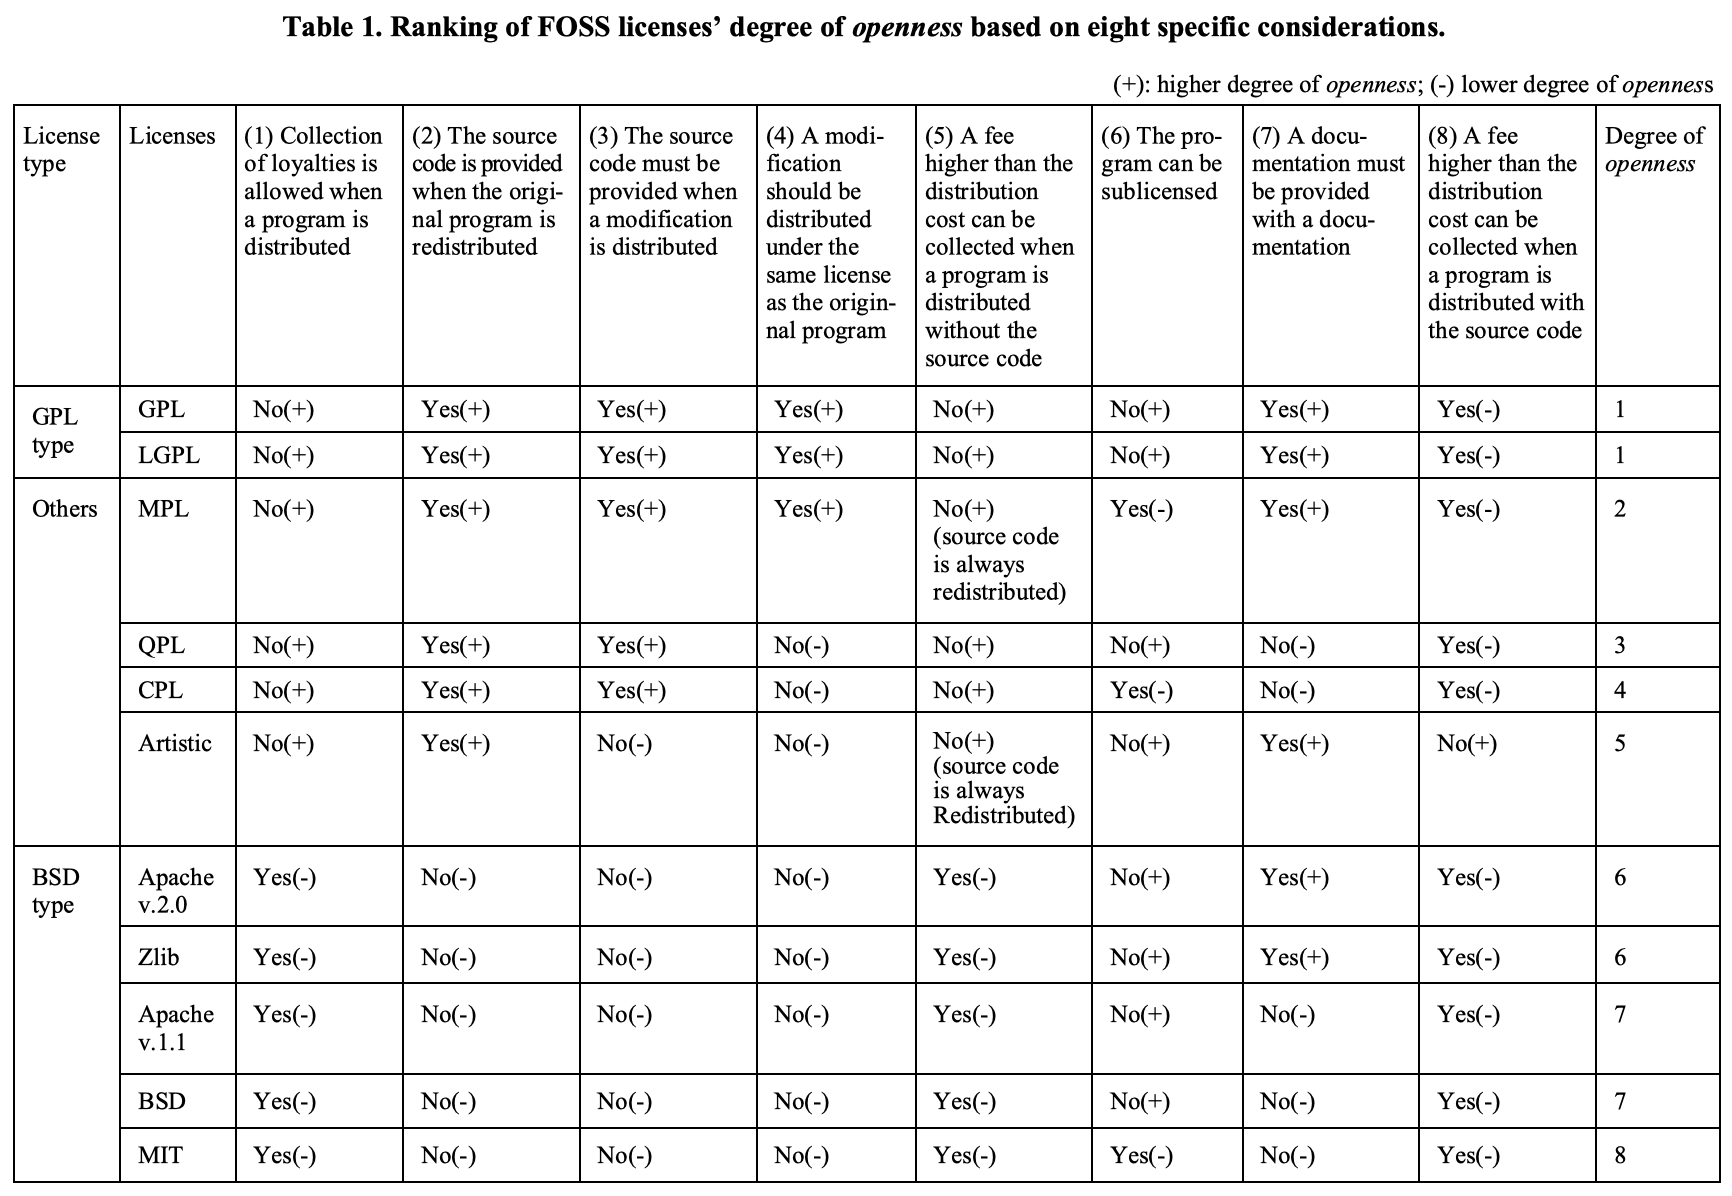
\includegraphics[width=.6\linewidth]{openness.png}
  \source{lin2006open}}

\qte
  [Ben Balter]
  {ben-balter}
  {Unsurprisingly, \ul{MIT}, \ul{Apache}, and \ul{GPL} are the clear front runners, with some 15\% of licensed projects opting for a non-standard license.}
  {github2015licenses}
\pitch{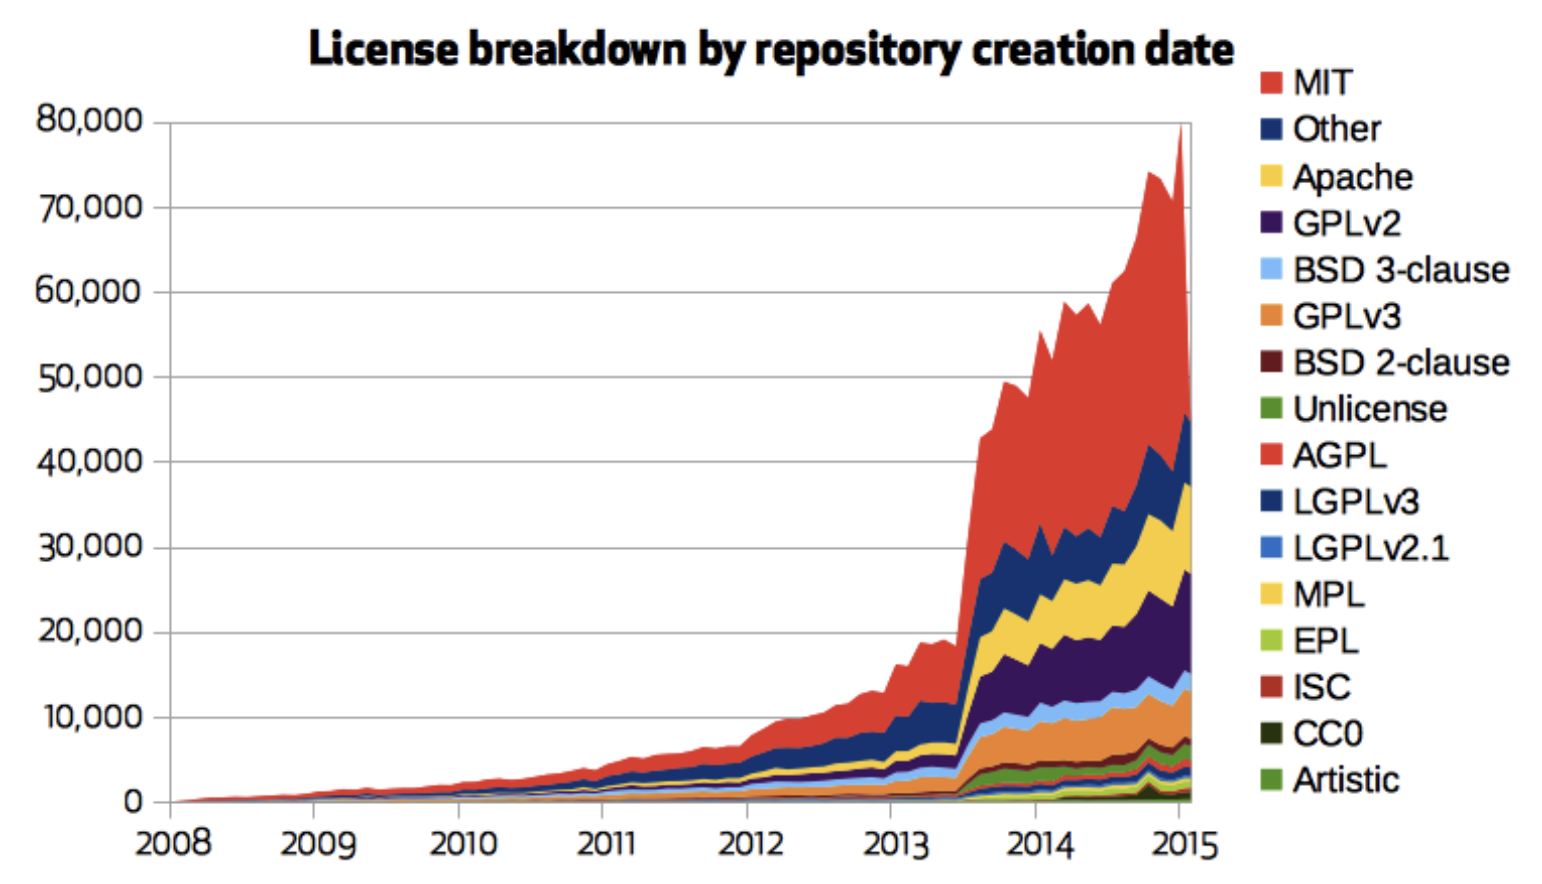
\includegraphics[width=.8\linewidth]{licenses.png}
  \source{github2015licenses}}

\thought[bugayenko2019blog0423]{Make the \ff{README.md} file attractive}

\plush{\pptBanner{Mandatory sections of \ff{README.md}:}
  \begin{itemize}
  \item Title, logo, badges
  \item What is it? What problem does it solve?
  \item How to uick start?
  \item How to contribute?
  \item Who is who?
  \end{itemize}
  \source{bugayenko2019blog0423}}

\qte
  [Gede Artha Azriadi Prana]
  {gede-prana}
  {We conduct a qualitative study involving the manual annotation of 4,226 README file sections from 393 randomly sampled GitHub repositories. We find that information discussing the `What' and `How' of a repository is very common, while many README files lack information regarding the purpose and status of a repository.}
  {prana2019categorizing}

\thought[bugayenko2014blog0721]{Make the \ff{master} branch read-only}

\thought{Don't explain coding guidelines, setup GitHub Action checks}

\thought{Put \ff{CODE\_OF\_CONDUCT.md} file to your repository... not}

\qte
  [Dabbish Laura]
  {dabbish-laura}
  {We found that projects in our sample \ul{did not} extensively discuss the addition or changes to the code of conduct.}
  {li2021code}

\qte
  [Jack Jamieson]
  {jack-jamieson}
  {We found multiple significant relationships between value-related discussions and turnover, including that discussions about \ul{respectfulness} predict an increase in contributors leaving and a decrease in new contributors, while discussions about \ul{social power} predicted better contributor retention.}
  {jamieson2023predicting}

\end{document}
